\section{Basic derivative rules} \label{S:2.4.BasicRules}

\begin{goals}
\item What are alternate notations for the derivative?
\item How can we sometimes use the algebraic structure of a function $f(x)$ to easily compute a formula for $f'(x)$?
\item What is the derivative of a power function of the form $f(x) = x^n$?  What is the derivative of an exponential function of form $f(x) = a^x$?
\item If we know the derivative of $y = f(x)$, how is the derivative of $y = k f(x)$ computed, where $k$ is a constant?
\item If we know the derivatives of $y = f(x)$ and $y = g(x)$, how is the derivative of $y = f(x) + g(x)$ computed?
\item What do the graphs of $y = \sin(x)$ and $y = \cos(x)$ suggest as formulas for their respective derivatives?
\end{goals}

%-----------------------------------
% SUBSECTION INTRODUCTION
%-----------------------------------
\subsection*{Introduction}

So far in this chapter, we developed the concept of the derivative of a function.  We now know that the derivative $f'$ of a function $f$ measures the instantaneous rate of change of $f$ with respect to $x$ as well as the slope of the tangent line to $y=f(x)$ at any given value of $x$.  To date, we have focused primarily on interpreting the derivative graphically or, in the context of functions in a physical setting, as a meaningful rate of change.  To actually calculate the value of the derivative at a specific point, we have typically relied on the limit definition of the derivative.

In this section, we will investigate how the limit definition of the derivative
\[ f'(x) = \lim_{h \to 0} \frac{f(x+h)-f(x)}{h} \]
leads to interesting patterns and rules that enable us to quickly find a formula for $f'(x)$ based on the formula for $f(x)$ \emph{without} using the limit definition directly.  For example, we already know that if $f(x) = x$, then it follows that $f'(x) = 1$.  While we could use the limit definition of the derivative to confirm this, we know it to be true because $f(x)$ is a linear function with slope $1$ at every value of $x$.  One of our goals is to be able to take standard functions, say ones such as $g(x) = 4x^7 - \sin(x) + 3e^x$, and, based on the algebraic form of the function, be able to apply shortcuts to almost immediately determine the formula for $g'(x)$.

\begin{pa} \label{PA:2.4}
Functions of the form $f(x) = x^n$, where $n = 1, 2, 3, \ldots$, are often called \emph{power functions}.  The first two questions below revisit work we did earlier, and the following questions extend those ideas to higher powers of $x$.
\ba
	\item Use the limit definition of the derivative to find $f'(x)$ for $f(x) = x^2$.
	\item Use the limit definition of the derivative to find $f'(x)$ for $f(x) = x^3$.
	\item Use the limit definition of the derivative to find $f'(x)$ for $f(x) = x^4$.  (Hint: $(a+b)^4 = a^4 + 4a^3b + 6a^2b^2 + 4ab^3 + b^4$.  Apply this rule to $(x+h)^4$ within the limit definition.)
	\item Based on your work in (a), (b), and (c), what do you conjecture is the derivative of $f(x) = x^5$?  Of $f(x) = x^{13}$?
	\item Conjecture a formula for the derivative of $f(x) = x^n$ that holds for any positive integer $n$.  That is, given $f(x) = x^n$ where $n$ is a positive integer, what do you think is the formula for $f'(x)$? 
\ea
\end{pa} \afterpa % PREVIEW ACTIVITY

%------------------------------------------
% SUBSECTION SOME KEY NOTATION
%------------------------------------------
%\subsection*{Some Key Notation}

%In addition to our usual $f'$ notation for the derivative, there are other ways to symbolically denote the derivative of a function, as well as the instruction to take the derivative.  We know that if we have a function, say  $f(x) = x^2$, that we can denote its derivative by $f'(x)$, and we write $f'(x) = 2x$.  Equivalently, if we are thinking more about the relationship between $y$ and $x$, we sometimes denote the derivative of $y$ with respect to $x$ with the symbol 
%$$\frac{dy}{dx}$$
%which we read ``dee-y dee-x.''  This notation comes from the fact that the derivative is related to the slope of a line, and slope is measured by $\frac{\triangle y}{\triangle x}$.  Note that while we read $\frac{\triangle y}{\triangle x}$ as ``change in $y$ over change in $x$,'' for the derivative symbol $\frac{dy}{dx}$, we view this is a single symbol, not a quotient of two quantities\footnote{That is, we do \emph{not} say ``dee-y over dee-x.''}.  For example, if $y = x^2$, we'll write that the derivative is $\frac{dy}{dx} = 2x.$

%Furthermore, we use a variant of $\frac{dy}{dx}$ notation to convey the instruction to take the derivative of a certain quantity with respect to a given variable.  In particular, if we write
%$$\frac{d}{dx}\left[ \Box \right]$$
%this means ``take the derivative of the quantity in $\Box$ with respect to $x$.''  To continue our example above with the squaring function, here we may write $\frac{d}{dx}[x^2] = 2x.$

%It is important to note that the independent variable can be different from $x$.  If we have $f(z) = z^2$, we then write $f'(z) = 2z$.  Similarly, if $y = t^2$, we can say $\frac{dy}{dt} = 2t$.  And changing the variable and derivative notation once more, it is also true that $\frac{d}{dq}[q^2] = 2q$.  This notation may also be applied to second derivatives:  $f''(z) =  \frac{d}{dz}\left[\frac{df}{dz}\right] = \frac{d^2 f}{dz^2}$.

%In what follows, we'll be working to widely expand our repertoire of functions for which we can quickly compute the corresponding derivative formula

%-----------------------------------------------------------------------------
% SUBSECTION CONSTANT, POWER, AND EXPONENTIAL FUNCTIONS
%-----------------------------------------------------------------------------
\subsection*{Constant, Power, and Exponential Functions}

So far, we have worked with the derivative formula for two important classes of functions:  constant functions and power functions.  For the first kind, observe that if $f(x) = c$ is a constant function, then its graph is a horizontal line with slope zero at every point.  Thus, $\frac{d}{dx}[c] = 0$.  We summarize this with the following rule.

\concept{Constant Rule \index{derivative!constant function}}{ % CONCEPT
For any real number $c$, if $f(x) = c$, then 
\[ f'(x) = 0. \]
} % end concept
Thus, if $f(x) = 7$, then $f'(x) = 0$.  Similarly, $\frac{d}{dx} [\sqrt{3}] = 0.$ 

\marginnote{The proof of the Constant Rule is found by applying the definition of the derivative, see Exercise~\ref{E:2.4-45}.}

For power functions, from your work in Preview Activity~\ref{PA:2.1}, you have conjectured that for any positive integer $n$, if $f(x) = x^n$, then $f'(x) = nx^{n-1}$.  Not only can this rule be formally proved to hold for any positive integer $n$ (see Activity~\ref{A:2.4.Act6}), but also for any nonzero real number (see Section~\ref{S:2.8.Inverse}).  

\concept{Power Rule \index{derivative!power function}}{ % CONCEPT
For any nonzero real number, if $f(x) = x^n$, then 
\[ f'(x) = nx^{n-1}. \]
} % end concept

This rule for power functions allows us to find derivatives such as the following:  if $g(z) = z^{-3}$, then $g'(z) = -3z^{-4}$.  Similarly, if $h(t) = t^{7/5}$, then $\frac{dh}{dt} = \frac{7}{5}t^{2/5}$; likewise, $\frac{d}{dq} [q^{\pi}] = \pi q^{\pi - 1}$. 

\begin{activity} \label{A:2.4.Act6}
Let $f(x) = x^n$, where $n$ is a positive integer.  The goal of this problem is to prove the Power Rule for derivatives, that we used in earlier work in this section.
\ba
\item State the Binomial Theorem.

\item Using the Binomial Theorem, expand $(x + h)^n$ for some positive integer $n$.

\item Use the limit definition of the derivative along with the Binomial Theorem to show that
\[ f'(x) = \lim_{h \to 0} \dfrac{x^n+nx^{n-1}h + \frac{n(n-1)}{2}x^{n-2}h^2 \cdots h^n - x^n}{h}. \]

\item Simplify the numerator of the derivative so that each term is multiplied by some expression in terms of $h$.

\item Reduce and compute the limit using algebra.
\ea

\end{activity}  % ACTIVITY need to write--Use binomial theorem to prove power rule for positive integers.

As we next turn to thinking about derivatives of combinations of basic functions, it will be instructive to have one more type of basic function whose derivative formula we know.  For now, we simply state this rule without explanation or justification; we will explore why this rule is true in Activity~\ref{A:2.4.Act5}, first we will encounter graphical reasoning for why the rule is plausible in Activity~\ref{A:2.4.Act4}.

\begin{marginfigure}[8cm]
\margingraphics{figures/2_2_PA1a.eps}
\caption{At left, the graph of $y = g(x) = 2^x$. At right, axes for plotting $y = g'(x)$.} \label{fig:2.4.Act4}
\end{marginfigure}

\begin{activity} \label{A:2.4.Act4}
Consider the function $g(x) = 2^x$, which is graphed in Figure~\ref{fig:2.4.Act4}.
\ba
	\item At each of $x = -2, -1, 0, 1, 2$, use a straightedge to sketch an accurate tangent line to $y = g(x)$.
	\item Use the provided grid to estimate the slope of the tangent line you drew at each point in (a).
	\item Use the limit definition of the derivative to estimate $g'(0)$ by using small values of $h$, and compare the result to your visual estimate for the slope of the tangent line to $y = g(x)$ at $x = 0$ in (b).
	\item Based on your work in (a), (b), and (c), sketch an accurate graph of $y = g'(x)$ on the axes adjacent to the graph of $y = g(x)$.
	\item Write at least one sentence that explains why it is reasonable to think that $g'(x) = cg(x)$, where $c$ is a constant.  In addition, calculate $\ln(2)$, and then discuss how this value, combined with your work above, reasonably suggests that $g'(x) = 2^x \ln(2)$.
\ea

\end{activity} %\afterpa % ACTIVITY Active preview 2.2

\concept{Exponential Rule \index{derivative!exponential function}}{ %CONCEPT
For any positive real number $a$, if $f(x) = a^x$, then 
\[ f'(x) = a^x \ln(a). \]
} % end concept

For instance, this rule tells us that if $f(x) = 2^x$, then $f'(x) = 2^x \ln(2)$.  Similarly, for $p(t) = 10^t$, $p'(t) = 10^t \ln(10)$.  It is especially important to note that when $a = e$, where $e$ is the base of the natural logarithm function, we have that 
$$\frac{d}{dx} [e^x] = e^x \ln(e) = e^x$$
since $\ln(e) = 1$.  This is an extremely important property of the function $e^x$:  its derivative function is itself!

\begin{activity} \label{A:2.4.Act5}
Let $f(x) = a^x$.  The goal of this problem is to explore how the value of $a$ affects the derivative of $f(x)$, without assuming we know the rule for $\frac{d}{dx}[a^x]$ that we have stated and used in earlier work in this section.
\ba
	\item Use the limit definition of the derivative to show that
	$$f'(x) = \lim_{h \to 0} \frac{a^x \cdot a^h - a^x}{h}.$$
	\item Explain why it is also true that
	$$f'(x) = a^x \cdot \lim_{h \to 0} \frac{a^h - 1}{h}.$$
	\item Use computing technology and small values of $h$ to estimate the value of 
	$$L = \lim_{h \to 0} \frac{a^h - 1}{h}$$
	when $a = 2$.  Do likewise when $a = 3$.
	\item Note that it would be ideal if the value of the limit $L$ was $1$, for then $f$ would be a particularly special function:  its derivative would be simply $a^x$, which would mean that its derivative is itself.  By experimenting with different values of $a$ between $2$ and $3$, try to find a value for $a$ for which 
	$$L = \lim_{h \to 0} \frac{a^h - 1}{h} = 1.$$
	\item Compute $\ln(2)$ and $\ln(3)$.  What does your work in (b) and (c) suggest is true about $\frac{d}{dx}[2^x]$ and $\frac{d}{dx}[2^x]$.
	\item How do your investigations in (d) lead to a particularly important fact about the number $e$?
\ea

\end{activity}  % ACTIVITY 

Finally, note carefully the distinction between power functions  and exponential functions:  in power functions, the variable is in the base, as in $x^2$, while in exponential functions, the variable is in the power, as in $2^x$.  As we can see from the rules, this makes a big difference in the form of the derivative.

The following activity will check your understanding of the derivatives of the three basic types of functions noted above.

\begin{activity} \label{A:2.1.1}  Use the three rules above to determine the derivative of each of the following functions.  For each, state your answer using full and proper notation, labeling the derivative with its name.  For example, if you are given a function $h(z)$, you should write ``$h'(z) = $'' or ``$\frac{dh}{dz} = $'' as part of your response.

\bmthree
\ba
	\item $\ds f(t) = \pi$
	\item $\ds g(z) = 7^z$
	\item $\ds h(w) = w^{3/4}$
	\item $\ds p(x) = 3^{1/2}$
	\item $\ds r(t) = (\sqrt{2})^t$
	\item $\ds \frac{d}{dq}[q^{-1}]$
	\item $\ds m(t) = \frac{1}{t^3}$
\ea
\emthree

\end{activity}
\begin{smallhint}
\ba
	\item Is $\pi$ a variable or a constant?
	\item Is $g$ a power or exponential function?
	\item Is $h$ a power or exponential function?
	\item Is $3^{1/2}$ a constant or a variable?
	\item $\sqrt{2}$ is a constant
	\item Remember the notation here means ``take the derivative with respect to $q$ of $q^{-1}$.''
	\item Rewrite the fraction using a negative exponent.
\ea
\end{smallhint}
\begin{bighint}
\ba
	\item Note that $\pi$ is a constant.
	\item Observe that $g$ an exponential function.
	\item $h$ is a power function.
	\item $3^{1/2}$ is a constant.
	\item $\sqrt{2}$ is a constant, so $r$ is an exponential function.
	\item Remember the notation here means ``take the derivative with respect to $q$ of $q^{-1}$.''  Note that $q{-1}$ is a power function.
	\item Recall that $\frac{1}{t^3} = t^{-3}$.
\ea
\end{bighint}
\begin{activitySolution}
\ba
	\item $f(t) = \pi$ is constant, so $f'(t) = 0$.
	\item $g(z) = 7^z$ is an exponential function, so $g'(z) = 7^z \ln(7)$.
	\item $h(w) = w^{3/4}$ is a power function, thus $h'(w) = \frac{3}{4} w^{-1/4}$.
	\item $p(x) = 3^{1/2}$ is constant, and therefore $\frac{dp}{dx} = 0$.
	\item $r(t) = (\sqrt{2})^t$ is exponential (since $\sqrt{2}$ is a constant), and so we have $r'(t) = (\sqrt{2})^t \ln (\sqrt{2})$.
	\item $\frac{d}{dq}[q^{-1}] = -q^{-2}$, by the rule for power functions.
	\item $m(t) = \frac{1}{t^3} = t^{-3}$, so $\frac{dm}{dt} = -3t^{-4} = -\frac{3}{t^4}$.
\ea
\end{activitySolution}
\aftera % ACTIVITY

%---------------------------------------------------------------------------
% SUBSECTION CONSTANT MULTIPLES AND SUMS OF FUNCTIONS
%---------------------------------------------------------------------------
\subsection*{Constant Multiples and Sums of Functions}

Of course, most of the functions we encounter in mathematics are more complicated than being simply constant, a power of a variable, or a base raised to a variable power.  In this section and several following, we will learn how to quickly compute the derivative of a function constructed as an algebraic combination of basic functions.  For instance, we'd like to be able to understand how to take the derivative of a polynomial function such as $p(t) = 3t^5 - 7t^4 + t^2 - 9$, which is a function made up of constant multiples and sums of powers of $t$.  To that end, we develop two new rules:  the Constant Multiple Rule and the Sum Rule.

Say we have a function $y = f(x)$ whose derivative formula is known.  How is the derivative of $y = kf(x)$ related to the derivative of the original function?  Recall that when we multiply a function by a constant $k$, we vertically stretch the graph by a factor of $|k|$ (and reflect the graph across $y = 0$ if $k < 0$).  This vertical stretch affects the slope of the graph, making the slope of the function $y = kf(x)$ be $k$ times as steep as the slope of $y = f(x)$.  In terms of the derivative, this is essentially saying that when we multiply a function by a factor of $k$, we change the value of its derivative by a factor of $k$ as well.  Thus, the Constant Multiple Rule holds:

\concept{The Constant Multiple Rule \index{constant multiple rule}}{ % CONCEPT
For any real number $k$, if $f(x)$ is a differentiable function with derivative $f'(x)$, then 
\[ \frac{d}{dx}[k f(x)] = k f'(x). \]
} % end concept

\marginnote{The Constant Multiple Rule can be formally proved as a consequence of properties of limits, using the limit definition of the derivative, see Exercise~\ref{E:2.4-46}}

In words, this rule says that ``the derivative of a constant times a function is the constant times the derivative of the function.''  For example, if $g(t) = 3 \cdot 5^t$, we have $g'(t) = 3 \cdot 5^t \ln(5)$.  Similarly, $\frac{d}{dz} [5z^{-2}] = 5 (-2z^{-3})$.

Next we examine what happens when we take a sum of two functions.  If we have $y = f(x)$ and $y = g(x)$, we can compute a new function $y = (f+g)(x)$ by adding the outputs of the two functions:  $(f+g)(x) = f(x) + g(x)$.  Not only does this result in the value of the new function being the sum of the values of the two known functions, but also the slope of the new function is the sum of the slopes of the known functions.  Therefore,  we arrive at the following Sum Rule for derivatives:

\concept{ The Sum Rule\index{sum rule}}{
If $f(x)$ and $g(x)$ are differentiable functions with derivatives $f'(x)$ and $g'(x)$ respectively, then 
\[ \frac{d}{dx}[f(x) + g(x)] = f'(x) + g'(x). \]
} % end concept

\marginnote{Like the Constant Multiple Rule, the Sum Rule can be formally proved as a consequence of properties of limits, using the limit definition of the derivative, see Exercise~\ref{E:2.4-47}.}

In words, the Sum Rule tells us that ``the derivative of a sum is the sum of the derivatives.''  It also tells us that any time we take a sum of two differentiable functions, the result must also be differentiable.  Furthermore, because we can view the difference function $y = (f-g)(x) = f(x) - g(x)$ as $y = f(x) + (-1 \cdot g(x))$, the Sum Rule and Constant Multiple Rules together tell us that $\frac{d}{dx}[f(x) + (-1 \cdot g(x))] = f'(x) - g'(x)$, or that ``the derivative of a difference is the difference of the derivatives.''  Hence we can now compute derivatives of sums and differences of elementary functions.  For instance, $\frac{d}{dw} (2^w + w^2) = 2^w \ln(2) + 2w$, and if $h(q) = 3q^6 - 4q^{-3}$, then $h'(q) = 3 (6q^5) - 4(-3q^{-4}) = 18q^5 + 12q^{-4}$.

\newpage

\begin{activity} \label{A:2.1.2}  Use only the rules for constant, power, and exponential functions, together with the Constant Multiple and Sum Rules,  to compute the derivative of each function below with respect to the given independent variable.  Note well that we do not yet know any rules for how to differentiate the product or quotient of functions.  This means that you may have to do some algebra first on the functions below before you can actually use existing rules to compute the desired derivative formula.  In each case, label the derivative you calculate with its name using proper notation such as $f'(x)$, $h'(z)$, $dr/dt$, etc.

\setlength{\columnsep}{5pt}
\bmtwo
\ba
	  \item $\ds f(x) = x^{5/3} - x^4 + 2^x$
	  \item $\ds g(x) = 14e^x + 3x^5 - x$
	  \item $\ds h(z) = \sqrt{z} + \frac{1}{z^4} + 5^z$
	  \item $\ds r(t) = \sqrt{53} \, t^7 - \pi e^t + e^4$
	  \item $\ds s(y) = (y^2 + 1)(y^2 - 1)$
	  \item $\ds q(x) = \ds \frac{x^3 - x + 2}{x}$
	  \item $\ds p(a) = 3a^4 - 2a^3 + 7a^2 - a + 12$
\ea
\emtwo

\end{activity}
\begin{smallhint}
\ba
	  \item Use the sum rule.
	  \item Use the sum rule together with the constant multiple rule.
	  \item How can you rewrite $\sqrt{z}$ using exponents?
	  \item Is $e^4$ a constant or variable?
	  \item Expand the product before attempting to find the derivative.
	  \item Rewrite the single fraction as a sum of three fractions, and simplify.
	  \item Note that ``$a$'' is the independent variable.
\ea
\end{smallhint}
\begin{bighint}
\ba
	  \item Use the sum rule; think about which functions in the sum are power functions and which are exponential.
	  \item Use the sum rule together with the constant multiple rule.  Note which functions are exponential and which are powers of $x$.
	  \item Recall that $\sqrt{z} = z^{1/2}$; also rewrite $\frac{1}{z^4}$ as a power of $z$.
	  \item Note that $\sqrt{53}$, $\pi$, and $e^4$ are all constants.
	  \item Expand the product and combine like terms before attempting to find the derivative.
	  \item Rewrite the single fraction as a sum of three fractions, and simplify.  That is, note that $q(x) = \ds \frac{x^3 - x + 2}{x} = \ds \frac{x^3}{x} - \frac{x}{x} + \frac{2}{x}$
	  \item Note that ``$a$'' is the independent variable and $p(a)$ is simply a polynomial in $a$.
\ea
\end{bighint}
\begin{activitySolution}
\ba
	  \item $f(x) = x^{5/3} - x^4 + 2^x$, so by the sum rule, $f'(x) = \frac{5}{3}x^{2/3} - 4 x^3 + 2^x \ln(2).$
	  \item $g(x) = 14e^x + 3x^5 - x$, so by the sum and constant multiple rules, $g'(x) = 14e^x + 3 \cdot 5x^4 - 1$.
	  \item $h(z) = \sqrt{z} + \frac{1}{z^4} + 5^z = z^{1/2} + z^{-4} + 5^z$, thus $h'(z) = \frac{1}{2}z^{-1/2} - 4z^{-5} + 5^z \ln(5)$.
	  \item Since $r(t) = \sqrt{53} \, t^7 - \pi e^t + e^4$ and $\sqrt{53}$, $\pi$, and $e^4$ are all constants, it follows from the sum and constant multiple rules, as well as the derivative of a constant rule, that $\frac{dr}{dt} = \sqrt{53} \cdot 7 t^6 - \pi e^t$.  (Note particularly that $\frac{d}{dt}[e^4] = 0$ since $e^4$ is constant.
	  \item $s(y) = (y^2 + 1)(y^2 - 1)= y^4 - 1$, thus $\frac{ds}{dy} = 4y^3$.
	  \item $q(x) = \ds \frac{x^3 - x + 2}{x} = \ds \frac{x^3}{x} - \frac{x}{x} + \frac{2}{x} = x^2 - 1 + 2x^{-1}$.  Now it follows that $q'(x) = 2x - 2x^{-2}$.
	  \item $p(a) = 3a^4 - 2a^3 + 7a^2 - a + 12$, so $p'(a) = 12a^3 - 6 a^2 + 14a - 1.$
\ea
\end{activitySolution}
\aftera % ACTIVITY

In the same way that we have shortcut rules to help us find derivatives, we introduce some language that is simpler and shorter.  Often, rather than say ``take the derivative of $f$,'' we'll instead say simply ``differentiate $f$.''  This phrasing is tied to the notion of having a derivative to begin with:  if the derivative exists at a point, we say ``$f$ is differentiable,'' which is tied to the fact that $f$ can be differentiated.

As we work more and more with the algebraic structure of functions, it is important to strive to develop a big picture view of what we are doing.  Here, we can note several general observations based on the rules we have so far.  One is that the derivative of any polynomial function will be another polynomial function, and that the degree of the derivative is one less than the degree of the original function.  For instance, if $p(t) = 7t^5 - 4t^3 + 8t$, $p$ is a degree $5$ polynomial, and its derivative, $p'(t) = 35t^4 - 12t^2 + 8$, is a degree $4$ polynomial.  Additionally, the derivative of any exponential function is another exponential function: for example, if $g(z) = 7 \cdot 2^z$, then $g'(z) = 7 \cdot 2^z \ln(2)$, which is also exponential.

Furthermore, while our current emphasis is on learning shortcut rules for finding derivatives without directly using the limit definition, we should be certain not to lose sight of the fact that all of the meaning of the derivative still holds that we developed earlier in this chapter.  That is, anytime we compute a derivative, that derivative measures the instantaneous rate of change of the original function, as well as the slope of the tangent line at any selected point on the curve.  The following activity asks you to combine the just-developed derivative rules with some key perspectives that we studied earlier.

\begin{activity} \label{A:2.4.3}  
Each of the following questions asks you to use derivatives to answer key questions about functions.  Be sure to think carefully about each question and to use proper notation in your responses.
\ba
	\item Find the slope of the tangent line to $h(z) = \sqrt{z} + \frac{1}{z}$ at the point where $z = 4$.
	\item A population of cells is growing in such a way that its total number in millions is given by the function $P(t) = 2(1.37)^t + 32$, where $t$ is measured in days.  
	\begin{enumerate}
	  \item[i.] Determine the instantaneous rate at which the population is growing on day $4$, and include units on your answer.  
	  \item[ii.] Is the population growing at an increasing rate or growing at a decreasing rate on day $4$?  Explain.
	\end{enumerate}
	\item Find an equation for the tangent line to the curve $p(a) = 3a^4 - 2a^3 + 7a^2 - a + 12$ at the point where $a=-1$.
	\item What is the difference between being asked to find the \emph{slope} of the tangent line (asked in (a)) and the \emph{equation} of the tangent line (asked in (c))?
\ea
\end{activity}
\begin{smallhint}
\ba
	  \item How would $h'(z)$ help you answer the question?
	  \item Think about finding both $P'(t)$ and $P''(t)$.
	  \item What two important pieces of information do you need to know to determine the equation of a line?
	  \item What information do you find in both (a) and (c)?
\ea
\end{smallhint}
\begin{bighint}
\ba
	  \item Remember that $h'(a)$ tells us the slope of the tangent line to $y = h(z)$ at the point $(a,h(a))$.
	  \item Think about how the units on $P'(t)$ are the units of $P$ per unit of $t$.  For the second question, consider the meaning of $P''(t)$.
	  \item Find both $(-1,p(-1))$ and $p'(-1)$.
	  \item Note that both questions require you to find the value of the given function's derivative at a particular point.  How is that value used differently in questions (a) and (c)?
\ea
\end{bighint}
\begin{activitySolution}
\ba
	  \item Note that since $h(z) = z^{1/2} + z^{-1}$, we have $h'(z) = \frac{1}{2}z^{-1/2} - z^{-2}$.  Thus, $h'(4) = \frac{1}{2(4)^{1/2}} - \frac{1}{4^2} = \frac{1}{4} - \frac{1}{16} = \frac{3}{16}.$  Thus, the slope of the tangent line to $h(z)$ at the point where $z = 4$ is $\frac{3}{16}$.
	  \item For (i.), note that $P'(t) = 2(1.37)^t \ln(1.37)$, and therefore $P'(4) =  2(1.37)^4 \ln(1.37) \approx 2.218$ million cells per day.  For (ii.), we can compute $P''(t)$ and find that $P''(t) = 2(1.37)^t \ln(1.37) \ln(1.37)$ and therefore find that $P''(4) \approx  0.69825$.  Since $P''(4)$ is positive, this tells us that the instantaneous rate of change $P'(t)$ is increasing at $t = 4$, and thus the population is growing at an increasing rate.
	  \item Given $p(a) = 3a^4 - 2a^3 + 7a^2 - a + 12$, first observe that $p(-1) = 3 + 2 + 7 + 1 + 12 = 25$, so the tangent line will pass through $(-1,25)$.  Further, since $p'(a) = 12a^3 - 6a^2 + 14a - 1$, we have $p'(-1) = -12 - 6 - 14 - 1 = -33$, which is the slope of the tangent line.  The equation of the tangent line is therefore $y - 25 = -33(a+1)$.
	  \item The biggest difference is that (a) asks for the \emph{slope} of the tangent line, while (c) asks for the \emph{equation} of the tangent line.  The latter requires the slope of the tangent line, but the slope and equation are two different entities.
\ea
\end{activitySolution}
\aftera % ACTIVITY

%---------------------------------------------------------------------------
% SUBSECTION THE SINE AND COSINE FUNCTIONS
%---------------------------------------------------------------------------
\subsection*{The sine and cosine functions}

The sine and cosine functions are among the most important functions in all of mathematics.  Sometimes called the \emph{circular} functions due to their genesis in the unit circle%\footnote{See Appendix * for a brief review of important trigonometry.}
, these periodic functions play a key role in modeling repeating phenomena such as the location of a point on a bicycle tire, the behavior of an oscillating mass attached to a spring, tidal elevations, and more.  Like polynomial and exponential functions, the sine and cosine functions are considered basic functions, ones that are often used in the building of more complicated functions.  As such, we would like to know formulas for $\frac{d}{dx} [\sin(x)]$ and $\frac{d}{dx} [\cos(x)]$, and the next two activities lead us to that end.



%\vspace{-1.5cm}

\begin{activity} \label{A:2.4.7}  Consider the function $f(x) = \sin(x)$, which is graphed in Figure~\ref{F:2.4.A7}.  Note carefully that the grid in the diagram does not have boxes that are $1 \times 1$, but rather approximately $1.57 \times 1$, as the horizontal scale of the grid is $\pi/2$ units per box.
\ba
	\item At each of $x = -2\pi, -\frac{3\pi}{2}, -\pi, -\frac{\pi}{2}, 0, \frac{\pi}{2}, \pi, \frac{3\pi}{2}, 2\pi,$ use a straightedge to sketch an accurate tangent line to $y = f(x)$.
	\item Use the provided grid to estimate the slope of the tangent line you drew at each point.  Pay careful attention to the scale of the grid.
	\item Use the limit definition of the derivative to estimate $f'(0)$ by using small values of $h$, and compare the result to your visual estimate for the slope of the tangent line to $y = f(x)$ at $x = 0$ in (b).  Using periodicity, what does this result suggest about $f'(2\pi)$?  about $f'(-2\pi)$?  
	\item Based on your work in (a), (b), and (c), sketch an accurate graph of $y = f'(x)$ on the axes adjacent to the graph of $y = f(x)$.
	\item What familiar function do you think is the derivative of $f(x) = \sin(x)$?
\ea
\end{activity}

\vspace{-1cm}

\begin{figure*} %FIGURE MAY NEED TO BE FULLWIDTH?
\begin{flushleft}
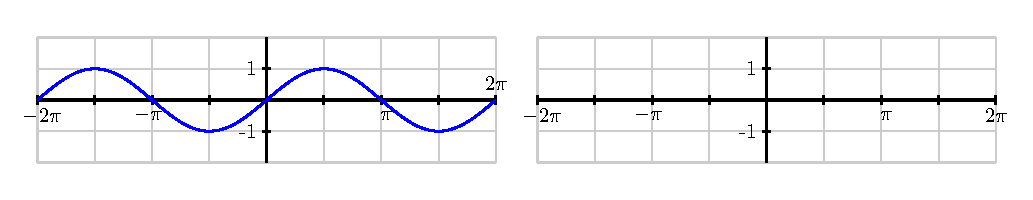
\includegraphics{figures/2_2_sine.eps}
\caption{At left, the graph of $y = f(x) = \sin(x)$.} \label{F:2.4.A7}
\end{flushleft}
\end{figure*}

\begin{smallhint}
\ba
	\item It's very important to use a straightedge for accuracy.
	\item First determine the slopes that appear to be zero.  Then estimate $f'(0)$ carefully using the grid.  Use symmetry and periodicity to help you estimate other nonzero slopes on the graph.
	\item $f'(0) \approx \frac{\sin(h)}{h}$ for small values of $h$. 
	\item Recall that heights on $f'$ come from slopes on $f$.
	\item It might be reasonable to expect that the derivative of a trigonometric function is another trigonometric function.
\ea
\end{smallhint}
\begin{bighint}
\ba
	\item It's very important to use a straightedge for accuracy.
	\item $f'(0) \approx 1$, as for each grid box we move horizontally, we go up about 1.5 grid boxes.
	\item $f'(0) \approx \frac{\sin(h)}{h}$ for small values of $h$.  Try using $h = 0.001$ and $h = -.001$. 
	\item Recall that heights on $f'$ come from slopes on $f$.  From your earlier work, you should know several places $f'(x) = 0$, plus that $f'(0) \approx 1$.  Plot these values on the grid for $y = f'(x)$.
	\item It might be reasonable to expect that the derivative of a trigonometric function is another trigonometric function, or possibly some multiple of such a function.
\ea 
\end{bighint}
\begin{activitySolution}
\ba
	\item See the figure below.
	\item Reading left to right from $-2\pi, \ldots, 2\pi$ with stepsize $\pi/2$, the respective slopes of tangent lines appear to be $1,0,-1,0,1,0,-1,0,1$.
	\item From the limit definition,
	\begin{eqnarray*}
	f'(0) & = & \lim_{h \to 0} \frac{f(0 + h) - f(0)}{h} \\
	       & = & \lim_{h \to 0} \frac{\sin(0 + h) - \sin(0)}{h} \\
	       & = & \lim_{h \to 0} \frac{\sin(h)}{h} 
	\end{eqnarray*}
	Because we cannot simplify the fraction $\frac{\sin(h)}{h}$ any further algebraically, we estimate the value of the limit using small values of $h$.  Doing so, it appears that $\lim_{h \to 0} \frac{\sin(h)}{h}  = 1$, and thus $f'(0) = 1$.  This matches the estimate generated visually by sketching the tangent line at $(0,f(0))$.  Finally, by the periodicity of the sine function, we expect the value of the derivative at 0 to match the derivative value at $-2\pi$ and $2\pi$.
	\item See the figure below.
	\item It appears that $\frac{d}{dx}[\sin(x)] = \cos(x)$.
\ea
%\begin{figure}[h]
\begin{center}
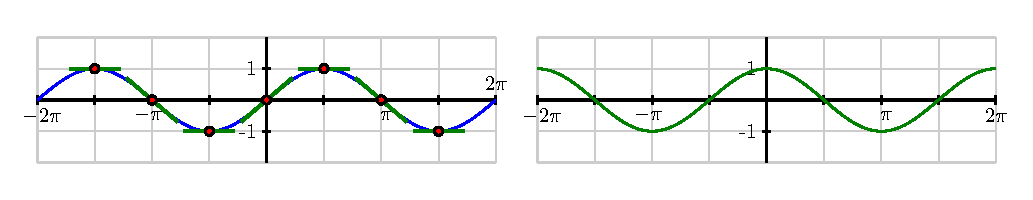
\includegraphics{figures/2_2_sineSoln.eps} %SOLUTION FIGURE??
%\caption{At left, the graph of $y = f(x) = \sin(x)$ along with several tangent lines.  At right, the graph of $y = f'(x)$, where the heights on the graph of $f'(x)$ come from slopes on the graph of $f$.} \label{F:2.2.A1Soln}
\end{center}
%\end{figure}
\end{activitySolution}
\aftera %ACTIVITY

\vspace{-.5cm}

\begin{activity} \label{A:2.4.Act8}  Consider the function $g(x) = \cos(x)$, which is graphed in Figure~\ref{F:2.4.A8}.  Note carefully that the grid in the diagram does not have boxes that are $1 \times 1$, but rather approximately $1.57 \times 1$, as the horizontal scale of the grid is $\pi/2$ units per box.

\ba
	\item At each of $x = -2\pi, -\frac{3\pi}{2}, -\pi, -\frac{\pi}{2}, 0, \frac{\pi}{2}, \pi, \frac{3\pi}{2}, 2\pi,$ use a straightedge to sketch an accurate tangent line to $y = g(x)$.
	\item Use the provided grid to estimate the slope of the tangent line you drew at each point.  Again, note the scale of the axes and grid.
	\item Use the limit definition of the derivative to estimate $g'(\frac{\pi}{2})$ by using small values of $h$, and compare the result to your visual estimate for the slope of the tangent line to $y = g(x)$ at $x = \frac{\pi}{2}$ in (b).  Using periodicity, what does this result suggest about $g'(-\frac{3\pi}{2})$?  can symmetry on the graph help you estimate other slopes easily?  
	\item Based on your work in (a), (b), and (c), sketch an accurate graph of $y = g'(x)$ on the axes adjacent to the graph of $y = g(x)$.
	\item What familiar function do you think is the derivative of $g(x) = \cos(x)$?
\ea
\end{activity}

\vspace{-1cm}

\begin{figure*}
\begin{flushleft}
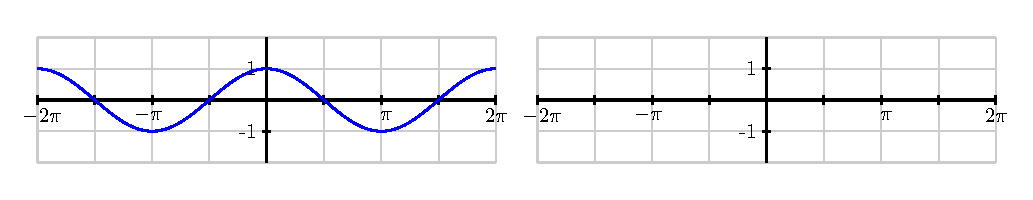
\includegraphics{figures/2_2_cosine.eps}
\caption{At left, the graph of $y = g(x) = \cos(x)$.} \label{F:2.4.A8}
\end{flushleft}
\end{figure*}

\begin{smallhint}
\ba
	\item It's very important to use a straightedge for accuracy.
	\item First determine the slopes that appear to be zero.  Then estimate $g'(\frac{\pi}{2})$ carefully using the grid.  Use symmetry and periodicity to help you estimate other nonzero slopes on the graph.
	\item $g'(\frac{\pi}{2}) \approx \frac{\cos(\frac{\pi}{2}+h)}{h}$ for small values of $h$. 
	\item Recall that heights on $g'$ come from slopes on $g$.
	\item It might be reasonable to expect that the derivative of a trigonometric function is another trigonometric function.
\ea
\end{smallhint}
\begin{bighint}
\ba
	\item It's very important to use a straightedge for accuracy.
	\item $g'(\frac{\pi}{2}) \approx -1$, as for each grid box we move horizontally, we go down about 1.5 grid boxes.
	\item $g'(\frac{\pi}{2}) \approx \frac{\cos(\frac{\pi}{2}+h)}{h}$ for small values of $h$.  Try using $h = 0.001$ and $h = -.001$. 
	\item Recall that heights on $g'$ come from slopes on $g$.  From your earlier work, you should know several places $g'(x) = 0$, plus that $g'(0) \approx 1$.  Plot these values on the grid for $y = g'(x)$.
	\item It might be reasonable to expect that the derivative of a trigonometric function is another trigonometric function, or possibly some multiple of such a function.
\ea 
\end{bighint}
\begin{activitySolution}
\ba
	\item See the figure below.
	\item Reading left to right from $-2\pi, \ldots, 2\pi$ with stepsize $\pi/2$, the respective slopes of tangent lines appear to be $0,-1,0,1,0,-1,0,1,0$.
	\item From the limit definition,
	\begin{eqnarray*}
	g'(\frac{\pi}{2}) & = & \lim_{h \to 0} \frac{g(\frac{\pi}{2} + h) - g(\frac{\pi}{2})}{h} \\
	       & = & \lim_{h \to 0} \frac{\cos(\frac{\pi}{2} + h) - \cos(\frac{\pi}{2})}{h} \\
	       & = & \lim_{h \to 0} \frac{\cos(\frac{\pi}{2}h)}{h} 
	\end{eqnarray*}
	Because we cannot simplify the fraction $\frac{\cos(\frac{\pi}{2}+h)}{h}$ any further algebraically, we estimate the value of the limit using small values of $h$.  Doing so, it appears that $\lim_{h \to 0} \frac{\cos(\frac{\pi}{2}+h)}{h}  = -1$, and thus $g'(\frac{\pi}{2}) = -1$.  This matches the estimate generated visually by sketching the tangent line at $(\frac{\pi}{2},g(\frac{\pi}{2}))$.  Finally, by the periodicity of the sine function, we expect the value of the derivative at $\frac{\pi}{2}$ to match the derivative value at $-\frac{3\pi}{2}$.
	\item See the figure below.
	\item It appears that $\frac{d}{dx}[\cos(x)] = -\sin(x)$.
\ea
%\begin{figure}[h]
\begin{center}
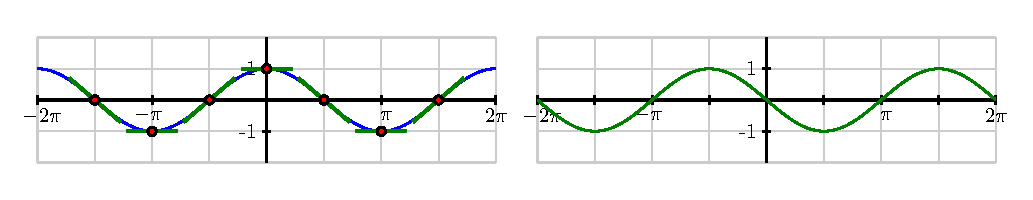
\includegraphics{figures/2_2_cosineSoln.eps} %FIGURE SOLN???
%\caption{At left, the graph of $y = f(x) = \sin(x)$ along with several tangent lines.  At right, the graph of $y = f'(x)$, where the heights on the graph of $f'(x)$ come from slopes on the graph of $f$.} \label{F:2.2.A1Soln}
\end{center}
%\end{figure}
\end{activitySolution}
\aftera %ACTIVITY

The results of the two preceding activities suggest that the sine and cosine functions not only have the beautiful interrelationships that are learned in a course in trigonometry -- connections such as the identities $\sin^2(x) + \cos^2(x) = 1$ and $\cos(x - \frac{\pi}{2}) = \sin(x)$ -- but that they are even further linked through calculus, as the derivative of each involves the other.  The following rules summarize the results of the activities. 

\concept{Sine and Cosine Functions \index{derivative!sine} \index{derivative!cosine}}{ For all real numbers $x$,  $$\frac{d}{dx} [\sin(x)] = \cos(x) \ \ \mbox{and} \ \ \frac{d}{dx} [\cos(x)] = -\sin(x)$$
} % end concept

\marginnote[-1cm]{These two rules may be formally proved using the limit definition of the derivative and the expansion identities for $\sin(x+h)$ and $\cos(x+h)$, see Activity-\ref{A:2.4.Act9}.}

\begin{activity} \label{A:2.4.Act9}  
In this problem, we explore how the limit definition of the derivative more formally shows that $\frac{d}{dx}[\sin(x)] = \cos(x)$.   Letting $f(x) = \sin(x)$, note that the limit definition of the derivative tells us that
	$$f'(x) = \lim_{h \to 0} \frac{\sin(x+h) - \sin(x)}{h}.$$
\ba
	\item Recall the trigonometric identity for the sine of a sum of angles $\alpha$ and $\beta$: $\sin(\alpha + \beta) = \sin(\alpha)\cos(\beta) + \cos(\alpha)\sin(\beta)$.  Use this identity and some algebra to show that
	$$f'(x) = \lim_{h \to 0} \frac{\sin(x)(\cos(h)-1) + \cos(x)\sin(h)}{h}.$$
	\item Next, note that as $h$ changes, $x$ remains constant. Explain why it therefore makes sense to say that
	$$f'(x) = \sin(x) \cdot \lim_{h \to 0} \frac{\cos(h) -1 }{h} + \cos(x) \cdot \lim_{h \to 0} \frac{\sin(h)}{h}.$$
	\item Finally, use small values of $h$ to estimate the values of the two limits in (c):
	$$\lim_{h \to 0} \frac{\cos(h) - 1}{h} \ \ \mbox{and} \ \ \lim_{h \to 0} \frac{\sin(h)}{h}.$$
	\item What do your results in (c) thus tell you about $f'(x)$?
	\item By emulating the steps taken above, use the limit definition of the derivative to argue convincingly that $\frac{d}{dx}[\cos(x)] = -\sin(x).$
\ea 

\end{activity}
%\begin{smallhint}
%\ba
%	\item Recall the constant multiple and sum rules.
%	\item $f'(\frac{\pi}{6})$ tells us the slope of the tangent line at $(\frac{\pi}{6},\frac{\pi}{6})$.
%	\item Find both $(\frac{\pi}{2}, g(\frac{\pi}{2}))$ and $g'(\frac{\pi}{2})$.
%	\item $\sin(\frac{\pi}{2})$ is a constant.
%	\item $P'(a)$ tells us the instantaneous rate of change of $P$ with respect to time at the instant $t = a$, and its units are ``units of $P$ per unit of time.''
%\ea
%\end{smallhint}
%\begin{bighint}
%\ba
%	\item Recall the constant multiple and sum rules.
%	\item $f'(a)$ tells us the slope of the tangent line at $(a,f(a))$.
%	\item Find both a point on the tangent line and the slope of the tangent line.
%	\item $\sin(\frac{\pi}{2})$ is a constant.
%	\item $P'(a)$ tells us the instantaneous rate of change of $P$ with respect to time at the instant $t = a$.
%\ea
%\end{bighint}
%\begin{activitySolution}
%\ba
%	\item By the sum and constant multiple rules, $\frac{dh}{dt} = 3(-\sin(t)) - 4(\cos(t)) = -3\sin(t) - 4\cos(t)$.
%	\item The exact slope of the tangent line to $y = f(x) = 2x + \frac{\sin(x)}{2}$ at $x = \frac{\pi}{6}$ is given by $f'(\frac{\pi}{6})$.  So, we first compute $f'(x)$.  Using the sum and constant multiple rules, $f'(x) = 2 + \frac{1}{2}\cos(x)$, and thus $f'(\frac{\pi}{6}) = 2 + \frac{1}{2} \cos(\frac{\pi}{6}) = 2 + \frac{\sqrt{3}}{4}.$
%	\item The tangent line passes through the point $(\frac{\pi}{2}, g(\frac{\pi}{2}))$ with slope $g'(\frac{\pi}{2})$.  We observe first that $g(\frac{\pi}{2}) = (\frac{\pi}{2})^2 + 2\cos(\frac{\pi}{2}) = \frac{\pi^2}{4}$.  Next, we compute the derivative function, $g'(x)$, and find that
%	$$g'(x) = 2x - 2\sin(x).$$
%	Thus, $g(\frac{\pi}{2}) = 2 \cdot \frac{\pi}{2} - 2 \sin(\frac{\pi}{2}) = \pi - 1$.
%	
%	Hence the equation of the tangent line (in point-slope form) is given by 
%	$$y - \frac{\pi^2}{4} = (\pi-1)(x-\frac{\pi}{2}).$$
%	\item Noting that $\sin(\frac{\pi}{2})$ is a constant, we have $p'(z) = 4z^3 + 4^z \ln(4) - 4\sin(z)$.
	
%	\item The value of $P'(2)$ will tell us the instantaneous rate of change of $P$ at the instant two decades have elapsed.  Observe that $P'(t) = 8\cos(t)$, and thus $P'(2) = 8\cos(2) \approx -3.329$ hundred animals per decade.  This tells us that the instantaneous rate of change of $P$ on January 1, 2030 is about $-3329$ animals per decade, which tells us that the animal population is shrinking considerably at this point in time.  We might say that for whatever the population is on January 1, 2030, we expect that population to drop by about 3300 animals over the next ten years, provided the current population trend continues.
%\ea
%\end{activitySolution}
\aftera %ACTIVITY

We have now added two additional functions to our library of basic functions whose derivatives we know: power functions, exponential functions, and the sine and cosine functions.  The constant multiple and sum rules still hold, of course, and all of the inherent meaning of the derivative persists, regardless of the functions that are used to constitute a given choice of $f(x)$.  The following activity puts our new knowledge of the derivatives of $\sin(x)$ and $\cos(x)$ to work.

\begin{activity} \label{A:2.4.Act10}  Answer each of the following questions.  Where a derivative is requested, be sure to label the derivative function with its name using proper notation.
\ba
	\item Determine the derivative of $h(t) = 3\cos(t) - 4\sin(t)$.
	\item Find the exact slope of the tangent line to $y = f(x) = 2x + \frac{\sin(x)}{2}$ at the point where $x = \frac{\pi}{6}$.
	\item Find the equation of the tangent line to $y = g(x) = x^2 + 2\cos(x)$ at the point where $x = \frac{\pi}{2}$.
	\item Determine the derivative of $p(z) = z^4 + 4^z + 4\cos(z) - \sin(\frac{\pi}{2})$.
	\item The function $P(t) = 24 + 8\sin(t)$ represents a population of a particular kind of animal that lives on a small island, where $P$ is measured in hundreds and $t$ is measured in decades since January $1$, $2010$.  What is the instantaneous rate of change of $P$ on January $1$, $2030$?  What are the units of this quantity?  Write a sentence in everyday language that explains how the population is behaving at this point in time.
\ea

\end{activity}
\begin{smallhint}
\ba
	\item Recall the constant multiple and sum rules.
	\item $f'(\frac{\pi}{6})$ tells us the slope of the tangent line at $(\frac{\pi}{6},\frac{\pi}{6})$.
	\item Find both $(\frac{\pi}{2}, g(\frac{\pi}{2}))$ and $g'(\frac{\pi}{2})$.
	\item $\sin(\frac{\pi}{2})$ is a constant.
	\item $P'(a)$ tells us the instantaneous rate of change of $P$ with respect to time at the instant $t = a$, and its units are ``units of $P$ per unit of time.''
\ea
\end{smallhint}
\begin{bighint}
\ba
	\item Recall the constant multiple and sum rules.
	\item $f'(a)$ tells us the slope of the tangent line at $(a,f(a))$.
	\item Find both a point on the tangent line and the slope of the tangent line.
	\item $\sin(\frac{\pi}{2})$ is a constant.
	\item $P'(a)$ tells us the instantaneous rate of change of $P$ with respect to time at the instant $t = a$.
\ea
\end{bighint}
\begin{activitySolution}
\ba
	\item By the sum and constant multiple rules, $\frac{dh}{dt} = 3(-\sin(t)) - 4(\cos(t)) = -3\sin(t) - 4\cos(t)$.
	\item The exact slope of the tangent line to $y = f(x) = 2x + \frac{\sin(x)}{2}$ at $x = \frac{\pi}{6}$ is given by $f'(\frac{\pi}{6})$.  So, we first compute $f'(x)$.  Using the sum and constant multiple rules, $f'(x) = 2 + \frac{1}{2}\cos(x)$, and thus $f'(\frac{\pi}{6}) = 2 + \frac{1}{2} \cos(\frac{\pi}{6}) = 2 + \frac{\sqrt{3}}{4}.$
	\item The tangent line passes through the point $(\frac{\pi}{2}, g(\frac{\pi}{2}))$ with slope $g'(\frac{\pi}{2})$.  We observe first that $g(\frac{\pi}{2}) = (\frac{\pi}{2})^2 + 2\cos(\frac{\pi}{2}) = \frac{\pi^2}{4}$.  Next, we compute the derivative function, $g'(x)$, and find that
	$$g'(x) = 2x - 2\sin(x).$$
	Thus, $g(\frac{\pi}{2}) = 2 \cdot \frac{\pi}{2} - 2 \sin(\frac{\pi}{2}) = \pi - 1$.
	
	Hence the equation of the tangent line (in point-slope form) is given by 
	$$y - \frac{\pi^2}{4} = (\pi-1)(x-\frac{\pi}{2}).$$
	\item Noting that $\sin(\frac{\pi}{2})$ is a constant, we have $p'(z) = 4z^3 + 4^z \ln(4) - 4\sin(z)$.
	
	\item The value of $P'(2)$ will tell us the instantaneous rate of change of $P$ at the instant two decades have elapsed.  Observe that $P'(t) = 8\cos(t)$, and thus $P'(2) = 8\cos(2) \approx -3.329$ hundred animals per decade.  This tells us that the instantaneous rate of change of $P$ on January 1, 2030 is about $-3329$ animals per decade, which tells us that the animal population is shrinking considerably at this point in time.  We might say that for whatever the population is on January 1, 2030, we expect that population to drop by about 3300 animals over the next ten years, provided the current population trend continues.
\ea
\end{activitySolution}
\aftera %ACTIVITY

%-------------
% SUMMARY
%-------------
\begin{summary}
\item Given a differentiable function $y = f(x)$, we can express the derivative of $f$ in several different notations:  $f'(x)$, $\frac{df}{dx}$, $\frac{dy}{dx}$, and $\frac{d}{dx}[f(x)]$.
\item The limit definition of the derivative leads to patterns among certain families of functions that enable us to compute derivative formulas without resorting directly to the limit definition.  For example, if $f$ is a power function of the form $f(x) = x^n$, then $f'(x) = nx^{n-1}$ for any real number $n$ other than $0$.  This is called the Rule for Power Functions.
\item We have stated a rule for derivatives of exponential functions in the same spirit as the rule for power functions:  for any positive real number $a$, if $f(x) = a^x$, then $f'(x) = a^x \ln(a)$.
\item If we are given a constant multiple of a function whose derivative we know, or a sum of functions whose derivatives we know, the Constant Multiple and Sum Rules make it straightforward to compute the derivative of the overall function.  More formally, if $f(x)$ and $g(x)$ are differentiable with derivatives $f'(x)$ and $g'(x)$ and $a$ and $b$ are constants, then
$$\frac{d}{dx} \left[af(x) + bg(x)\right] = af'(x) + bg'(x).$$
\item If we consider the graph of an exponential function $f(x) = a^x$ (where $a > 1$), the graph of $f'(x)$ behaves similarly, appearing exponential and as a possibly scaled version of the original function $a^x$.  For $f(x) = 2^x$, careful analysis of the graph and its slopes suggests that $\frac{d}{dx}[2^x] = 2^x \ln(2)$.
\item By carefully analyzing the graphs of $y = \sin(x)$ and $y = \cos(x)$, plus using the limit definition of the derivative at select points, we found that $\frac{d}{dx} [\sin(x)] = \cos(x)$ and $\frac{d}{dx} [\cos(x)] = -\sin(x)$.
\end{summary}

\clearpage

%--------------
% EXERCISES
%--------------
\begin{adjustwidth*}{}{-2.25in}
\textbf{{\large Exercises}}
\setlength{\columnsep}{25pt}
\begin{multicols*}{2}
\noindent Terms and Concepts \small
\begin{enumerate}[1)]
\item What is the name of the rule which states that $\ds \frac{d}{dx}\big(x^n\big) = nx^{n-1}$, where $n>0$ is an integer?
\item Give an example of a function $f(x)$ where $f'(x) = f(x)$.
\item Give an example of a function $f(x)$ where $f'(x) = 0$.
\item The derivative rules introduced in this section explain how to compute the derivative of which of the following functions?

\setlength{\columnsep}{15pt}
\bmtwo
\ba
\item $\ds g(x) = 3x^2-x+17$ 
\item $\ds h(x) = 5\ln(x)$ 
\item $\ds j(x) = \sin(x) \cos(x)$ 
\item $\ds k(x) = e^{x^2}$
\item $\ds m(x) = \sqrt{x}$
\item $\ds f(x) = \frac{3}{x^2}$ 
\ea
\emtwo
\setlength{\columnsep}{25pt}
\end{enumerate} 

\noindent {\normalsize Problems} \small

\noindent {\bf In exercises 5--13, compute the derivative of the given function.}

\begin{enumerate}[1),resume]
\item $\ds f(x) = 7x^2-5x+7$
\item $\ds g(x) = 14x^3+7x^2+11x-29$
\item $\ds m(t) = 9t^5-\frac{1}{8}t^3+3t-8$
\item $\ds f(\theta) = 9\sin(\theta) + 10\cos(\theta)$
\item $\ds f(r) = 6e^r$
\item $\ds g(t) = 10t^4-\cos(t) +7\sin(t)$
\item $\ds p(s) = \frac{1}{4}s^4+\frac{1}{3}s^3+\frac{1}{2}s^2+s+1$
\item $\ds h(t) = e^t - \sin(t) - \cos(t)$
\item $\ds g(t) = (1+3t)^2$
\end{enumerate}

\noindent {\bf In exercises 14--19, compute the first four derivatives of the given function.}

\begin{enumerate}[1),resume]
\item $\ds f(x) = x^6$
\item $\ds g(x) = 2\cos(x)$
\item $\ds h(t) = t^2 - e^t$
\item $\ds p(\theta) = \theta^4-\theta^3$
\item $\ds f(\theta) = \sin(\theta)-\cos(\theta)$
\item $f(x)=1,100$
\end{enumerate}

\noindent {\bf In exercises 20--24, find the equation of the tangent line of the function at the given point.}

\begin{enumerate}[1),resume]
\item $\ds f(x)=x^3-x$ at $x=1$
\item $\ds f(t)=e^t+3$ at $t=0$
\item $\ds f(x)=4\sin(x)$ at $x=\pi/2$
\item $\ds f(x)=-2\cos(x)$ at $x=\pi/4$
\item $\ds f(x)=2x+3$ at $x=5$

\item Let $f$ and $g$ be differentiable functions for which the following information is known:  $f(2) = 5$, $g(2) = -3$, $f'(2) = -1/2$, $g'(2) = 2$.
\ba
	\item Let $h$ be the new function defined by the rule $h(x) = 3f(x) - 4g(x)$.  Determine $h(2)$ and $h'(2)$.
	\item Find an equation for the tangent line to $y = h(x)$ at the point $(2,h(2))$.
	\item Let $p$ be the function defined by the rule $p(x) = -2f(x) + \frac{1}{2}g(x)$.  Is $p$ increasing, decreasing, or neither at $a = 2$?  Why?
	\item Estimate the value of $p(2.03)$ by using the local linearization of $p$ at the point $(2,p(2))$.
\ea

\item Consider the functions $r(t) = t^t$ and $s(t) = \arccos(t)$, for which you are given the facts that $r'(t) = t^t(\ln(t) + 1)$ and $s'(t) = -\frac{1}{\sqrt{1-t^2}}$.  Do not be concerned with where these derivative formulas come from.  We restrict our interest in both functions to the domain $0 < t < 1$.
\ba
	\item Let $w(t) = 3t^t - 2\arccos(t)$.  Determine $w'(t)$.
	\item Find an equation for the tangent line to $y = w(t)$ at the point $(\frac{1}{2}, w(\frac{1}{2}))$.
	\item Let $v(t) = t^t + \arccos(t)$.  Is $v$ increasing or decreasing at the instant $t = \frac{1}{2}$?  Why?
\ea

\item Let functions $p$ and $q$ be the piecewise linear functions given by their respective graphs given below.  Use the graphs to answer the following questions.
\begin{center}
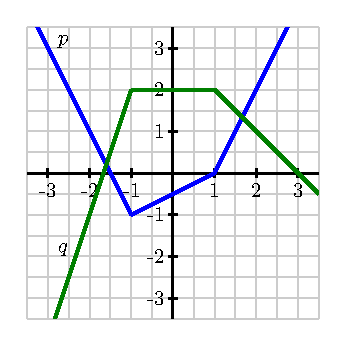
\includegraphics[scale=.7]{figures/2_1_Ez3.eps}
\end{center}
\ba
	\item At what values of $x$ is $p$ not differentiable?  At what values of $x$ is $q$ not differentiable? Why?
	\item Let $r(x) = p(x) + 2q(x)$.  At what values of $x$ is $r$ not differentiable? Why?
	\item Determine $r'(-2)$ and $r'(0)$.
	\item Find an equation for the tangent line to $y = r(x)$ at the point $(2,r(2))$.
\ea

\item Use the definition of the derivative to prove the Constant Rule for differentiation. \label{E:2.4-45}

\item Use the definition of the derivative to prove the Constant Multiple Rule for differentiation. \label{E:2.4-46}

\item Use the definition of the derivative to prove the Sum Rule for differentiation. \label{E:2.4-47}
\end{enumerate}

%------------------------------------------
% END OF EXERCISES ON FIRST PAGE
%------------------------------------------
\end{multicols*}
\end{adjustwidth*}

\afterexercises 

\cleardoublepage